\beginsong{Wenn die Bürger schlafen geh'n}[
    wuw={Theo Mackeben, Otto Ernst Hesse}, 
    jahr={1938}, 
    bo={378}, 
    siru={267},
    tonspur={596}, 
]

\beginverse
\endverse
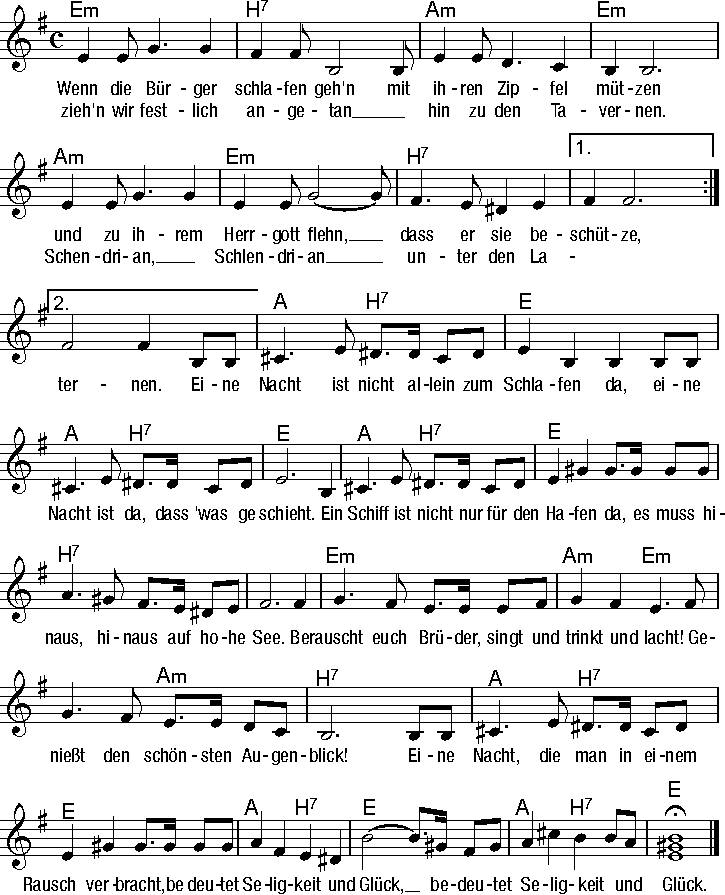
\includegraphics[draft=false, width=1\textwidth]{Noten/Lied096.pdf}

\beginverse
\[Em]Wenn im Glase \[H7]perlt der Sekt \[Am]unter roten \[Em]Ampeln,
\[Am]und die Weiber, \[Em]süß erschreckt, \[H7]auf dem Schoß uns trampeln,
\[Em]küssen wir die \[H7]Prüderie \[Am]von den roten \[Em]Mündern,
\[Am]Amnestie, \[Em]Amnestie \[H7]allen armen Sündern!
\endverse 

\beginchorus
Eine \[A]Nacht ist \[H7]nicht allein zum \[E]Schlafen da,eine \[A]Nacht ist da\[H7], dass was ge\[E]schieht. 
Ein \[A]Schiff ist \[H7]nicht nur für den \[E]Hafen da, es muss hi\[H7]naus, hinaus auf hohe See.
Be\[Em]rauscht euch Brüder, singt und \[Am]trinkt und \[Em]lacht! Genießt den \[Am]schönsten Augen\[H7]blick!
Eine \[A]Nacht, die \[H7]man in einem \[E]Rausch verbracht, \lrep bedeutet \[A]Selig\[H7]keit und \[E]Glück. \rrep
\endchorus


\beginverse
^Wenn die Morgen^dämmerung ^hinter Fenster^scheiben
^und die Männer ^ohne Braut ^beieinander bleiben,
^schmieden wir im ^Flüsterton ^aus Gesprächen ^Bomben.
^Rebellion, ^Rebellion ^in den Katakomben.
\endverse

\printchorus

\endsong

\beginscripture{}
Der 1938 veröffentlichte Schlager durfte auf Grund der dritten Strophe „Rebellion, Rebellion, in den Katakomben" in Deutschland nicht auf Platte veröffentlicht werden.
\endscripture
